\section{Introduction to Model-Based Testing}

\begin{itemize}

\item Testing is the most costly phase of a software development project.

\item We can use formal methods to make testing almost automatic.

\item Model-based testing uses a formal specification to generate test cases and to verify whether they found errors or not.

\item The following picture depicts the basic model-based testing methodology, which is based on:

\begin{itemize}
\item P. Stocks, ``Applying formal methods to software testing,'' Ph.D. dissertation, Department of Computer Science, University of Queensland, 1993.

\item H. M. Hörcher and J. Peleska, ``Using formal specifications to support software testing,'' {\it Software Quality Journal}, vol. 4, pp. 309--327, 1995.

\item P. Stocks and D. Carrington, ``A framework for specification-based testing,'' {\it IEEE Transactions on Software Engineering}, vol. 22, no. 11, pp. 777--793, Nov. 1996.
\end{itemize}

\end{itemize}

\begin{figure}[h]
\begin{center}
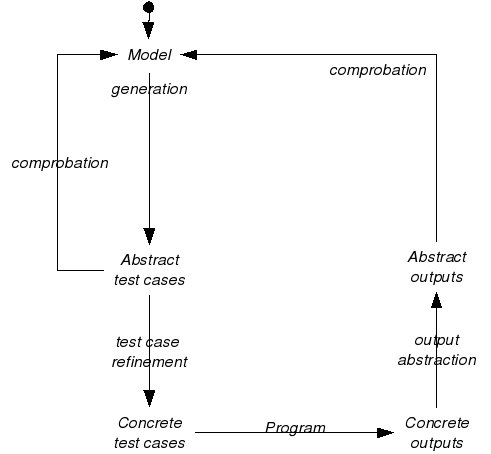
\includegraphics{/home/mcristia/fceia/software/Fastest/doc/testing-func-01.png} 
\caption{Model-based testing methodology: general view.}
\end{center}
\end{figure}


\begin{itemize}
%\item For the {\it refinement} step we defined a language to write {\it refinement functions}. 

%A refinement function translate abstract test cases (or abstract constants) into concrete test cases (i.e. written in C, Java or any other programming language). The language is purely declarative.

\item The following figure shows with more detail how the {\it generation} phase is composed.

\item The current version of FASTEST implements the {\it generation} phase but it does not include {\it pruning}. 

In a couple of month we'll release a version implementing also the {\it test case refinement} phase.

\end{itemize}

\begin{figure}[h]
\begin{center}
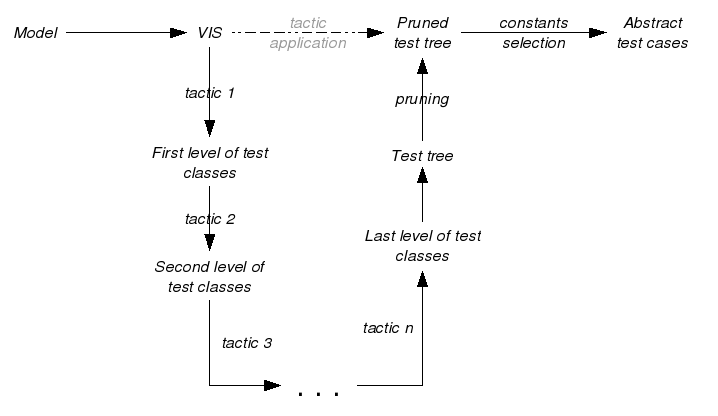
\includegraphics[scale=0.9]{/home/mcristia/fceia/software/Fastest/doc/testing-func-02.png}
\caption{Model-based testing methodology: detailed view of the {\it generation} phase and the {\it tactic application} step.}
\end{center}
\end{figure}

\begin{itemize}

\item Testing tactics\footnote{Stocks and Carrington use strategies instead of tactics.} are different ways of partitioning a set of abstract test cases.

\begin{itemize}
\item Disjunctive Normal Form, Standard Partitions, Sub-domain Propagation, Cause-Effect, Specification Mutation, etc.
\end{itemize}

\item Each tactic is applied over the last test tree level.

\item Test classes are sets of abstract test cases defined by comprehension, then each test class is identified by a predicate.

\item Test classes' predicates obey the relationship depicted in Figure \ref{tcp}.

\end{itemize}

\begin{figure}[h]
\setlength{\DTbaselineskip}{20pt}
\DTsetlength{1em}{3em}{0.1em}{1pt}{4pt}
\dirtree{%
 .1 $VIS$\DTcomment{$P$}.
 .2 $C_{1}^{T1}$\DTcomment{$P \land P_{1}^{1}$}.
 .2 $C_{2}^{T1}$\DTcomment{$P \land P_{2}^{1}$}.
 .3 $C_{1}^{T2}$\DTcomment{$P \land P_{2}^{1} \land P_{1}^{2}$}.
 .3 $C_{2}^{T2}$\DTcomment{$P \land P_{2}^{1} \land P_{2}^{2}$}.
 .2 $C_{3}^{T1}$\DTcomment{$P \land P_{3}^{1}$}.
 .3 $C_{3}^{T2}$\DTcomment{$P \land P_{3}^{1} \land P_{3}^{2}$}.
 .3 $C_{4}^{T2}$\DTcomment{$P \land P_{3}^{1} \land P_{4}^{2}$}.
 .4 $C_{1}^{T3}$\DTcomment{$P \land P_{3}^{1} \land P_{3}^{2} \land P_{1}^{3}$}.
 .4 $C_{2}^{T3}$\DTcomment{$P \land P_{3}^{1} \land P_{3}^{2} \land P_{2}^{3}$}.
}
\caption{\label{tcp}The predicate of a test class at some level is the conjunction of the predicate of its parent test class and a its own predicate.}
\end{figure}

\begin{itemize}

\item Abstract test cases are selected only from the leafs.

\item As a consequence, the deeper the tree, the more accurate and discovering the test cases.

\item Pruning the initial test tree saves time because many leafs are in fact empty sets (they represent impossible situations).

%\item For the constant selection phase we have applied reduction to finite models. 

\item A typical test tree with four levels of test classes is depicted in Figure \ref{ttt}.

\end{itemize}

\begin{figure}
\begin{center}
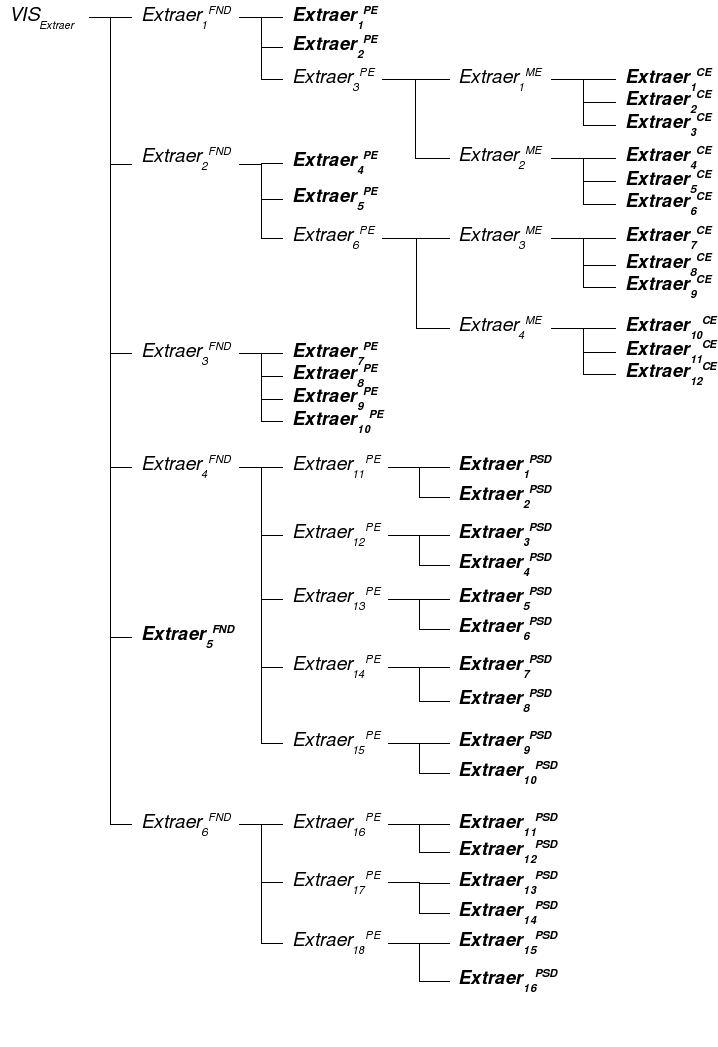
\includegraphics[scale=0.9]{/home/mcristia/fceia/software/Fastest/doc/testing-func-03.png}
\caption{\label{ttt}Example of a test tree with four levels of test classes.}
\end{center}
\end{figure}

\pagebreak

\section{FASTEST Architecture in a Nutshell}

\begin{itemize}

\item FASTEST architecture was guided by:

\begin{itemize}

\item Performance, because calculating thousands of test cases can be very time consuming;

\item Modificability, because we don't know yet what features industry could need; and

\item Documentability, because to test must mean to document.

\end{itemize}

\item Hence, we combined two different architectural styles and we used open formats and tools in our interfaces:

\begin{itemize}

\item Client/Server, so we distribute test case calculation;

\item Implicit Invocation, so we can add, modify and remove components as new and more sophisticated requirements arise;

\item Latex is used to read specifications and to generate test trees, test classes, abstract test cases, etc.;

\item FASTEST is integrated with the Community Z Tools (CZT, \verb+http://czt.sourceforge.net/+), to avoid duplicate efforts in programming core modules.

\end{itemize}

\item FASTEST' process structure is shown in Figure \ref{fep}.

\begin{figure}
\begin{center}
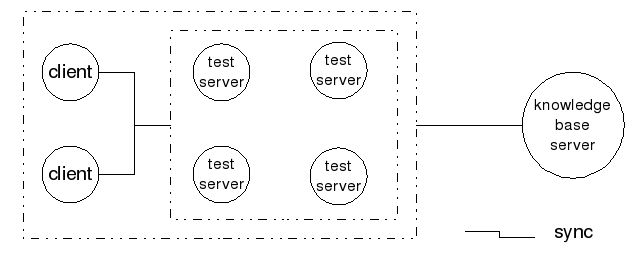
\includegraphics{/home/mcristia/fceia/software/Fastest/doc/fastest-ep.png}
\end{center}
\caption{\label{fep}FASTEST's process structure is composed by a number of clients and servers, and just one instance of a knowledge-base server.}
\end{figure}

\begin{itemize}
\item Clients interact with the user, generate test trees and run test cases. 

\item All of the other functions are performed on the servers.

\item The knowledge base server stores testing tactics, abstract test cases, refinement functions, etc. so testers can use them for re-testing within a given project and for testing in different projects.

Currently this server is no fully implemented.
\end{itemize}

\end{itemize}

\pagebreak

\section{An Example}

\begin{itemize}
\item We have said that model-based testing takes as input a formal model of the system to be tested.

\item FASTEST uses Z specifications. 

The current version does not support the full language. For instance, schema composition, schema piping, the theta operator, schema as types, axiomatic definitions and so on, are not supported yet.

\item The first goal is to apply FASTEST to unit testing; then we'll try to extend it to integration and system testing.

\item Then, say we have to test a function that must keep the highest readings from a set of sensors.

\end{itemize}

\subsection{The Z Formal Specification Language}

\begin{itemize}

\item Z is a formal notation useful to specify systems that will use complex data structures and will apply complex transformations over them.

\item It's a textual language based on first order logic and discrete mathematics.

\item A Z model is a state machine where states are defined by state variables and transitions are predicates over those variables.

\item The Z formal specification for the function mentioned above is as follows.

\item Note that we do not include state invariants in the state schema, but instead we find that writing them as proof obligations (like in the B method or TLA+) is a better practice. 

Actually we did not write the invariant in this example in order to simplify the presentation.
\end{itemize}

\begin{multicols}{2}
\begin{zed}
[SENSOR]
\end{zed}

\begin{zed}
MaxReadings == [smax: SENSOR \pfun \num]
\end{zed}

\begin{schema}{KeepMaxReadingOk}
\Delta MaxReadings \\
s?:SENSOR; r?:\num \\
\where
s? \in \dom smax \\
smax~s? < r?\\
smax' = smax \oplus \{s? \mapsto r?\}
%smax' = (\dom \{s? \mapsto r?\} \ndres smax) \oplus \{s? \mapsto r?\}
\end{schema}

\begin{zed}
KeepMaxReadingE1 == \\
  \t1 [\Xi MaxReadings; s?:SENSOR | \\
  \t1 s? \notin \dom smax]
\end{zed}

\begin{schema}{KeepMaxReadingE2}
\Xi MaxReadings \\
s?:SENSOR; r?:\num
\where
s? \in \dom smax\\
r? \leq smax~s? 
\end{schema}

\begin{zed}
KeepMaxReading == \\
  \t1 KeepMaxReadingOk \\
  \t1 \lor KeepMaxReadingE1 \\
  \t1 \lor KeepMaxReadingE2
\end{zed}


\end{multicols}

\subsection{Generating the Test Tree}

\begin{itemize}

\item The first step is to use FASTEST to generate the test tree.

\item The test tree depends on the tactics you apply and the order they are applied.

\item In this case we apply two testing tactics:

\begin{itemize}

\item Disjunctive Normal Form (DNF); it's applied by default.

\item Standard Partitions (SP), applied to the expression $smax~s? < r?$ present in schema $KeepMaxReadingOk$.

\end{itemize}

\item Then, the test tree is the one shown in Figure \ref{cstt}.

\end{itemize}

\begin{figure}
\dirtree{%
 .1 \hyperlink{s:KeepMaxReading\_VIS}{KeepMaxReading\_VIS}.
 .2 \hyperlink{s:KeepMaxReading\_DNF\_1}{KeepMaxReading\_DNF\_1}.
 .3 \hyperlink{s:KeepMaxReading\_SP\_1}{KeepMaxReading\_SP\_1}.
 .3 \hyperlink{s:KeepMaxReading\_SP\_2}{KeepMaxReading\_SP\_2}.
 .3 \hyperlink{s:KeepMaxReading\_SP\_3}{KeepMaxReading\_SP\_3}.
 .3 \hyperlink{s:KeepMaxReading\_SP\_4}{KeepMaxReading\_SP\_4}.
 .3 \hyperlink{s:KeepMaxReading\_SP\_5}{KeepMaxReading\_SP\_5}.
 .3 \hyperlink{s:KeepMaxReading\_SP\_6}{KeepMaxReading\_SP\_6}.
 .3 \hyperlink{s:KeepMaxReading\_SP\_7}{KeepMaxReading\_SP\_7}.
 .3 \hyperlink{s:KeepMaxReading\_SP\_8}{KeepMaxReading\_SP\_8}.
 .3 \hyperlink{s:KeepMaxReading\_SP\_9}{KeepMaxReading\_SP\_9}.
 .2 \hyperlink{s:KeepMaxReading\_DNF\_2}{KeepMaxReading\_DNF\_2}.
 .3 \hyperlink{s:KeepMaxReading\_SP\_10}{KeepMaxReading\_SP\_10}.
 .3 \hyperlink{s:KeepMaxReading\_SP\_11}{KeepMaxReading\_SP\_11}.
 .3 \hyperlink{s:KeepMaxReading\_SP\_12}{KeepMaxReading\_SP\_12}.
 .3 \hyperlink{s:KeepMaxReading\_SP\_13}{KeepMaxReading\_SP\_13}.
 .3 \hyperlink{s:KeepMaxReading\_SP\_14}{KeepMaxReading\_SP\_14}.
 .3 \hyperlink{s:KeepMaxReading\_SP\_15}{KeepMaxReading\_SP\_15}.
 .3 \hyperlink{s:KeepMaxReading\_SP\_16}{KeepMaxReading\_SP\_16}.
 .3 \hyperlink{s:KeepMaxReading\_SP\_17}{KeepMaxReading\_SP\_17}.
 .3 \hyperlink{s:KeepMaxReading\_SP\_18}{KeepMaxReading\_SP\_18}.
 .2 \hyperlink{s:KeepMaxReading\_DNF\_3}{KeepMaxReading\_DNF\_3}.
 .3 \hyperlink{s:KeepMaxReading\_SP\_19}{KeepMaxReading\_SP\_19}.
 .3 \hyperlink{s:KeepMaxReading\_SP\_20}{KeepMaxReading\_SP\_20}.
 .3 \hyperlink{s:KeepMaxReading\_SP\_21}{KeepMaxReading\_SP\_21}.
 .3 \hyperlink{s:KeepMaxReading\_SP\_22}{KeepMaxReading\_SP\_22}.
 .3 \hyperlink{s:KeepMaxReading\_SP\_23}{KeepMaxReading\_SP\_23}.
 .3 \hyperlink{s:KeepMaxReading\_SP\_24}{KeepMaxReading\_SP\_24}.
 .3 \hyperlink{s:KeepMaxReading\_SP\_25}{KeepMaxReading\_SP\_25}.
 .3 \hyperlink{s:KeepMaxReading\_SP\_26}{KeepMaxReading\_SP\_26}.
 .3 \hyperlink{s:KeepMaxReading\_SP\_27}{KeepMaxReading\_SP\_27}.
}


\caption{\label{cstt}Testing tree for $KeepMaxReading$.}
\end{figure}

\begin{itemize}

\item Each node in the test tree is also a Z schema, each of which describes the conditions for selecting test cases.
\end{itemize}

\begin{multicols}{2}
\begin{schema}{KeepMaxReading\_VIS}\\
 smax : SENSOR \pfun \num \\
 s? : SENSOR \\
 r? : \num 
\end{schema}


\begin{schema}{KeepMaxReading\_DNF\_1}\\
 smax : SENSOR \pfun \num \\
 s? : SENSOR \\
 r? : \num 
\where
 s? \in \dom smax \\
 smax~s? < r?
\end{schema}


\begin{schema}{KeepMaxReading\_SP\_1}\\
 smax : SENSOR \pfun \num \\
 s? : SENSOR \\
 r? : \num 
\where
 s? \in \dom smax \\
 smax~s? < r? \\
 smax~s? < 0 \\
 r? < 0
\end{schema}


\begin{schema}{KeepMaxReading\_SP\_2}
 smax : SENSOR \pfun \num \\
 s? : SENSOR \\
 r? : \num 
\where
 s? \in \dom smax \\
 smax~s? < r? \\
 smax~s? < 0 \\
 r? = 0
\end{schema}


\begin{schema}{KeepMaxReading\_SP\_3}\\
 smax : SENSOR \pfun \num \\
 s? : SENSOR \\
 r? : \num 
\where
 s? \in \dom smax \\
 smax~s? < r? \\
 smax~s? < 0 \\
 r? > 0
\end{schema}


\begin{schema}{KeepMaxReading\_SP\_4}\\
 smax : SENSOR \pfun \num \\
 s? : SENSOR \\
 r? : \num 
\where
 s? \in \dom smax \\
 smax~s? < r? \\
 smax~s? = 0 \\
 r? < 0
\end{schema}


\begin{schema}{KeepMaxReading\_SP\_5}\\
 smax : SENSOR \pfun \num \\
 s? : SENSOR \\
 r? : \num 
\where
 s? \in \dom smax \\
 smax~s? < r? \\
 smax~s? = 0 \\
 r? = 0
\end{schema}


\begin{schema}{KeepMaxReading\_SP\_6}\\
 smax : SENSOR \pfun \num \\
 s? : SENSOR \\
 r? : \num 
\where
 s? \in \dom smax \\
 smax~s? < r? \\
 smax~s? = 0 \\
 r? > 0
\end{schema}


\begin{schema}{KeepMaxReading\_SP\_7}\\
 smax : SENSOR \pfun \num \\
 s? : SENSOR \\
 r? : \num 
\where
 s? \in \dom smax \\
 smax~s? < r? \\
 smax~s? > 0 \\
 r? < 0
\end{schema}


\begin{schema}{KeepMaxReading\_SP\_8}\\
 smax : SENSOR \pfun \num \\
 s? : SENSOR \\
 r? : \num 
\where
 s? \in \dom smax \\
 smax~s? < r? \\
 smax~s? > 0 \\
 r? = 0
\end{schema}


\begin{schema}{KeepMaxReading\_SP\_9}\\
 smax : SENSOR \pfun \num \\
 s? : SENSOR \\
 r? : \num 
\where
 s? \in \dom smax \\
 smax~s? < r? \\
 smax~s? > 0 \\
 r? > 0
\end{schema}


\begin{schema}{KeepMaxReading\_DNF\_2}\\
 smax : SENSOR \pfun \num \\
 s? : SENSOR \\
 r? : \num 
\where
 s? \notin \dom smax
\end{schema}


\begin{schema}{KeepMaxReading\_SP\_10}\\
 smax : SENSOR \pfun \num \\
 s? : SENSOR \\
 r? : \num 
\where
 s? \notin \dom smax \\
 smax~s? < 0 \\
 r? < 0
\end{schema}


\begin{schema}{KeepMaxReading\_SP\_11}\\
 smax : SENSOR \pfun \num \\
 s? : SENSOR \\
 r? : \num 
\where
 s? \notin \dom smax \\
 smax~s? < 0 \\
 r? = 0
\end{schema}


\begin{schema}{KeepMaxReading\_SP\_12}\\
 smax : SENSOR \pfun \num \\
 s? : SENSOR \\
 r? : \num 
\where
 s? \notin \dom smax \\
 smax~s? < 0 \\
 r? > 0
\end{schema}


\begin{schema}{KeepMaxReading\_SP\_13}\\
 smax : SENSOR \pfun \num \\
 s? : SENSOR \\
 r? : \num 
\where
 s? \notin \dom smax \\
 smax~s? = 0 \\
 r? < 0
\end{schema}


\begin{schema}{KeepMaxReading\_SP\_14}\\
 smax : SENSOR \pfun \num \\
 s? : SENSOR \\
 r? : \num 
\where
 s? \notin \dom smax \\
 smax~s? = 0 \\
 r? = 0
\end{schema}


\begin{schema}{KeepMaxReading\_SP\_15}\\
 smax : SENSOR \pfun \num \\
 s? : SENSOR \\
 r? : \num 
\where
 s? \notin \dom smax \\
 smax~s? = 0 \\
 r? > 0
\end{schema}


\begin{schema}{KeepMaxReading\_SP\_16}\\
 smax : SENSOR \pfun \num \\
 s? : SENSOR \\
 r? : \num 
\where
 s? \notin \dom smax \\
 smax~s? > 0 \\
 r? < 0
\end{schema}


\begin{schema}{KeepMaxReading\_SP\_17}\\
 smax : SENSOR \pfun \num \\
 s? : SENSOR \\
 r? : \num 
\where
 s? \notin \dom smax \\
 smax~s? > 0 \\
 r? = 0
\end{schema}


\begin{schema}{KeepMaxReading\_SP\_18}\\
 smax : SENSOR \pfun \num \\
 s? : SENSOR \\
 r? : \num 
\where
 s? \notin \dom smax \\
 smax~s? > 0 \\
 r? > 0
\end{schema}


\begin{schema}{KeepMaxReading\_DNF\_3}\\
 smax : SENSOR \pfun \num \\
 s? : SENSOR \\
 r? : \num 
\where
 s? \in \dom smax \\
 r? \leq smax~s?
\end{schema}


\begin{schema}{KeepMaxReading\_SP\_19}\\
 smax : SENSOR \pfun \num \\
 s? : SENSOR \\
 r? : \num 
\where
 s? \in \dom smax \\
 r? \leq smax~s? \\
 smax~s? < 0 \\
 r? < 0
\end{schema}


\begin{schema}{KeepMaxReading\_SP\_20}\\
 smax : SENSOR \pfun \num \\
 s? : SENSOR \\
 r? : \num 
\where
 s? \in \dom smax \\
 r? \leq smax~s? \\
 smax~s? < 0 \\
 r? = 0
\end{schema}


\begin{schema}{KeepMaxReading\_SP\_21}\\
 smax : SENSOR \pfun \num \\
 s? : SENSOR \\
 r? : \num 
\where
 s? \in \dom smax \\
 r? \leq smax~s? \\
 smax~s? < 0 \\
 r? > 0
\end{schema}


\begin{schema}{KeepMaxReading\_SP\_22}\\
 smax : SENSOR \pfun \num \\
 s? : SENSOR \\
 r? : \num 
\where
 s? \in \dom smax \\
 r? \leq smax~s? \\
 smax~s? = 0 \\
 r? < 0
\end{schema}


\begin{schema}{KeepMaxReading\_SP\_23}\\
 smax : SENSOR \pfun \num \\
 s? : SENSOR \\
 r? : \num 
\where
 s? \in \dom smax \\
 r? \leq smax~s? \\
 smax~s? = 0 \\
 r? = 0
\end{schema}


\begin{schema}{KeepMaxReading\_SP\_24}\\
 smax : SENSOR \pfun \num \\
 s? : SENSOR \\
 r? : \num 
\where
 s? \in \dom smax \\
 r? \leq smax~s? \\
 smax~s? = 0 \\
 r? > 0
\end{schema}


\begin{schema}{KeepMaxReading\_SP\_25}\\
 smax : SENSOR \pfun \num \\
 s? : SENSOR \\
 r? : \num 
\where
 s? \in \dom smax \\
 r? \leq smax~s? \\
 smax~s? > 0 \\
 r? < 0
\end{schema}


\begin{schema}{KeepMaxReading\_SP\_26}\\
 smax : SENSOR \pfun \num \\
 s? : SENSOR \\
 r? : \num 
\where
 s? \in \dom smax \\
 r? \leq smax~s? \\
 smax~s? > 0 \\
 r? = 0
\end{schema}


\begin{schema}{KeepMaxReading\_SP\_27}\\
 smax : SENSOR \pfun \num \\
 s? : SENSOR \\
 r? : \num 
\where
 s? \in \dom smax \\
 r? \leq smax~s? \\
 smax~s? > 0 \\
 r? > 0
\end{schema}



\end{multicols}

\subsection{\label{fatc}Finding Abstract Test Cases}

\begin{itemize}

\item Now, FASTEST tries to find one abstract test case in each leaf of the testing tree.

\item Here FASTEST generates a finite model over which it evaluates each leaf's predicate.
\begin{itemize}
\item If some element of the finite model satisfies a test class' predicate, then we have found an abstract test case in that class.

\item If no element in the finite model satisfies the predicate, it can be due to two causes:

\begin{itemize}
\item The predicate is a contradiction (during pruning FASTEST could not determine that).

\item The finite model is not a appropriate.
\end{itemize}
\end{itemize}

\item Table \ref{summary} gives a summary of the search for abstract test cases for the present example.

\begin{table}
\begin{center}
\begin{tabular}{|c|c|c|c|c|} \hline
{\bf Leafs} & {\bf Found} & \multicolumn{3}{|c|}{{\bf Failed}} \\
 &  & \multicolumn{1}{c} {\bf Possible} & \multicolumn{1}{c}{\bf Impossible} & \multicolumn{1}{c|}{\bf Undefined} \\\hline
{\bf 27}    & {\bf 11}     & {\bf 0}      & {\bf 7}          & {\bf 9} \\\hline
\end{tabular}
\caption{\label{summary} Summary}
\end{center}
\end{table}


\begin{itemize}
\item {\bf (Possible)} In a first attempt, FASTEST failed to find abstract test cases for

\begin{multicols}{2}
\begin{schema}{KeepMaxReading\_ SP\_ 1}\\
 smax : SENSOR \pfun \num \\
 s? : SENSOR \\
 r? : \num 
\where
 s? \in \dom smax \\
 smax~s? < r? \\
 smax~s? < 0 \\
 r? < 0
\end{schema}

\begin{schema}{KeepMaxReading\_ SP\_ 9}\\
 smax : SENSOR \pfun \num \\
 s? : SENSOR \\
 r? : \num 
\where
 s? \in \dom smax \\
 smax~s? < r? \\
 smax~s? > 0 \\
 r? > 0
\end{schema}
\end{multicols}

because the default finite set for $\num$ is $\{-1,0,1\}$. 

However, if before instructing FASTEST to find abstract test cases, we instruct it to build other finite models for these test classes, then it will find the corresponding abstract test cases.

On the other hand, you have to take into consideration that FASTEST needs almost 9 hours to find a test case for $KeepMaxReading\_ SP\_ 9$. Future versions of FASTEST will dramatically improve on this.

\item {\bf (Impossible)} Most, if not all, the empty test classes can automatically be eliminated when the pruning step will be implemented.

\item {\bf (Undefined)} The nine undefined cases correspond to test classes where $s? \notin \dom smax$ is part of the predicate, because the predicate contains also the expression $smax~s?$ which is undefined when $s? \notin \dom smax$.

For these cases we have two options (we're still investigating which is the best). If $P$ is a predicate depending on $f~x$ and $x \notin \dom f$, then we can consider either:

\begin{itemize}
\item That $P(f~x)$ is false, in which case the test class containing $P$ is empty and should be pruned from the test tree.

\item That $P(f~x)$ is true regardless the value of $f~x$, in which case FASTEST should try to find an abstract test case in this test class but considering only the other predicates that define the class.
\end{itemize}

In any case it's rather easy to improve on these cases making FASTEST find either one or nine more abstract test cases.

\item {\bf In summary, future versions of FASTEST will automatically yield between 12 to 20 test cases for an operation like $KeepMaxReading$.}
\end{itemize}

\item The extended test tree, i.e. the test tree containing also the abstract test cases of the test classes for which it was possible to find one, is shown in Figure \ref{csett}.
\end{itemize}

\begin{figure}
\dirtree{%
 .1 \hyperlink{s:KeepMaxReading\_VIS}{KeepMaxReading\_VIS}.
 .2 \hyperlink{s:KeepMaxReading\_DNF\_1}{KeepMaxReading\_DNF\_1}.
 .3 \hyperlink{s:KeepMaxReading\_SP\_1}{KeepMaxReading\_SP\_1}.
 .4 \hyperlink{s:KeepMaxReading\_SP\_1\_TCASE}{KeepMaxReading\_SP\_1\_TCASE}.
 .3 \hyperlink{s:KeepMaxReading\_SP\_2}{KeepMaxReading\_SP\_2}.
 .4 \hyperlink{s:KeepMaxReading\_SP\_2\_TCASE}{KeepMaxReading\_SP\_2\_TCASE}.
 .3 \hyperlink{s:KeepMaxReading\_SP\_3}{KeepMaxReading\_SP\_3}.
 .4 \hyperlink{s:KeepMaxReading\_SP\_3\_TCASE}{KeepMaxReading\_SP\_3\_TCASE}.
 .3 \hyperlink{s:KeepMaxReading\_SP\_4}{KeepMaxReading\_SP\_4}.
 .3 \hyperlink{s:KeepMaxReading\_SP\_5}{KeepMaxReading\_SP\_5}.
 .3 \hyperlink{s:KeepMaxReading\_SP\_6}{KeepMaxReading\_SP\_6}.
 .4 \hyperlink{s:KeepMaxReading\_SP\_6\_TCASE}{KeepMaxReading\_SP\_6\_TCASE}.
 .3 \hyperlink{s:KeepMaxReading\_SP\_7}{KeepMaxReading\_SP\_7}.
 .3 \hyperlink{s:KeepMaxReading\_SP\_8}{KeepMaxReading\_SP\_8}.
 .3 \hyperlink{s:KeepMaxReading\_SP\_9}{KeepMaxReading\_SP\_9}.
 .4 \hyperlink{s:KeepMaxReading\_SP\_9\_TCASE}{KeepMaxReading\_SP\_9\_TCASE}.
 .2 \hyperlink{s:KeepMaxReading\_DNF\_2}{KeepMaxReading\_DNF\_2}.
 .3 \hyperlink{s:KeepMaxReading\_SP\_10}{KeepMaxReading\_SP\_10}.
 .3 \hyperlink{s:KeepMaxReading\_SP\_11}{KeepMaxReading\_SP\_11}.
 .3 \hyperlink{s:KeepMaxReading\_SP\_12}{KeepMaxReading\_SP\_12}.
 .3 \hyperlink{s:KeepMaxReading\_SP\_13}{KeepMaxReading\_SP\_13}.
 .3 \hyperlink{s:KeepMaxReading\_SP\_14}{KeepMaxReading\_SP\_14}.
 .3 \hyperlink{s:KeepMaxReading\_SP\_15}{KeepMaxReading\_SP\_15}.
 .3 \hyperlink{s:KeepMaxReading\_SP\_16}{KeepMaxReading\_SP\_16}.
 .3 \hyperlink{s:KeepMaxReading\_SP\_17}{KeepMaxReading\_SP\_17}.
 .3 \hyperlink{s:KeepMaxReading\_SP\_18}{KeepMaxReading\_SP\_18}.
 .2 \hyperlink{s:KeepMaxReading\_DNF\_3}{KeepMaxReading\_DNF\_3}.
 .3 \hyperlink{s:KeepMaxReading\_SP\_19}{KeepMaxReading\_SP\_19}.
 .4 \hyperlink{s:KeepMaxReading\_SP\_19\_TCASE}{KeepMaxReading\_SP\_19\_TCASE}.
 .3 \hyperlink{s:KeepMaxReading\_SP\_20}{KeepMaxReading\_SP\_20}.
 .3 \hyperlink{s:KeepMaxReading\_SP\_21}{KeepMaxReading\_SP\_21}.
 .3 \hyperlink{s:KeepMaxReading\_SP\_22}{KeepMaxReading\_SP\_22}.
 .4 \hyperlink{s:KeepMaxReading\_SP\_22\_TCASE}{KeepMaxReading\_SP\_22\_TCASE}.
 .3 \hyperlink{s:KeepMaxReading\_SP\_23}{KeepMaxReading\_SP\_23}.
 .4 \hyperlink{s:KeepMaxReading\_SP\_23\_TCASE}{KeepMaxReading\_SP\_23\_TCASE}.
 .3 \hyperlink{s:KeepMaxReading\_SP\_24}{KeepMaxReading\_SP\_24}.
 .3 \hyperlink{s:KeepMaxReading\_SP\_25}{KeepMaxReading\_SP\_25}.
 .4 \hyperlink{s:KeepMaxReading\_SP\_25\_TCASE}{KeepMaxReading\_SP\_25\_TCASE}.
 .3 \hyperlink{s:KeepMaxReading\_SP\_26}{KeepMaxReading\_SP\_26}.
 .4 \hyperlink{s:KeepMaxReading\_SP\_26\_TCASE}{KeepMaxReading\_SP\_26\_TCASE}.
 .3 \hyperlink{s:KeepMaxReading\_SP\_27}{KeepMaxReading\_SP\_27}.
 .4 \hyperlink{s:KeepMaxReading\_SP\_27\_TCASE}{KeepMaxReading\_SP\_27\_TCASE}.
}

\caption{\label{csett}The extended test tree includes also the schema boxes representing test cases hanging from those leafs for which FASTES was able to find a test case.}
\end{figure}

\begin{itemize}
\item Again, each abstract test case is a Z schema, but now each state and input variable equals a constant value.
\end{itemize}

\begin{multicols}{2}
\begin{schema}{KeepMaxReading\_SP\_1\_TCASE}\\
 KeepMaxReading\_SP\_1 
\where
 r? =~\negate 1 \\
 smax = \{ ( sensor0 , \negate 2 ) \} \\
 s? = sensor0
\end{schema}


\begin{schema}{KeepMaxReading\_SP\_2\_TCASE}\\
 KeepMaxReading\_SP\_2 
\where
 r? = 0 \\
 smax = \{ ( sensor0 , \negate 1 ) \} \\
 s? = sensor0
\end{schema}


\begin{schema}{KeepMaxReading\_SP\_3\_TCASE}\\
 KeepMaxReading\_SP\_3 
\where
 r? = 1 \\
 smax = \{ ( sensor0 , \negate 1 ) \} \\
 s? = sensor0
\end{schema}


\begin{schema}{KeepMaxReading\_SP\_6\_TCASE}\\
 KeepMaxReading\_SP\_6 
\where
 r? = 1 \\
 smax = \{ ( sensor0 , 0 ) \} \\
 s? = sensor0
\end{schema}


\begin{schema}{KeepMaxReading\_SP\_9\_TCASE}\\
 KeepMaxReading\_SP\_9 
\where
 r? = 2 \\
 smax = \{ ( sensor0 , 1 ) \} \\
 s? = sensor0
\end{schema}


\begin{schema}{KeepMaxReading\_SP\_19\_TCASE}\\
 KeepMaxReading\_SP\_19 
\where
 r? =~\negate 1 \\
 smax = \{ ( sensor0 , \negate 1 ) \} \\
 s? = sensor0
\end{schema}


\begin{schema}{KeepMaxReading\_SP\_22\_TCASE}\\
 KeepMaxReading\_SP\_22 
\where
 r? =~\negate 1 \\
 smax = \{ ( sensor0 , 0 ) \} \\
 s? = sensor0
\end{schema}


\begin{schema}{KeepMaxReading\_SP\_23\_TCASE}\\
 KeepMaxReading\_SP\_23 
\where
 r? = 0 \\
 smax = \{ ( sensor0 , 0 ) \} \\
 s? = sensor0
\end{schema}


\begin{schema}{KeepMaxReading\_SP\_25\_TCASE}\\
 KeepMaxReading\_SP\_25 
\where
 r? =~\negate 1 \\
 smax = \{ ( sensor0 , 1 ) \} \\
 s? = sensor0
\end{schema}


\begin{schema}{KeepMaxReading\_SP\_26\_TCASE}\\
 KeepMaxReading\_SP\_26 
\where
 r? = 0 \\
 smax = \{ ( sensor0 , 1 ) \} \\
 s? = sensor0
\end{schema}


\begin{schema}{KeepMaxReading\_SP\_27\_TCASE}\\
 KeepMaxReading\_SP\_27 
\where
 r? = 1 \\
 smax = \{ ( sensor0 , 1 ) \} \\
 s? = sensor0
\end{schema}



\end{multicols}


\subsection{The FASTEST Script}

The FASTEST script to do all the previous work is (assuming that file \verb+sensors-simp.tex+ is in the same directory than \verb+fastest.jar+, i.e. the installation directory):

\begin{verbatim}
$> java -jar fastest.jar
FASTest version 1.0, (C) 2008, Flowgate Security Consulting
FASTest>loadspec sensors-simp.tex
FASTest>selop KeepMaxReading
FASTest>addtactic KeepMaxReading SP < smax~s? < r?
FASTest>settcasestrategy Iterative KeepMaxReading_SP_1 4 -int Zero
FASTest>settcasestrategy Iterative KeepMaxReading_SP_9 5 -int Zero
FASTest>genalltca
FASTest>showtt
FASTest>showsch -tca
\end{verbatim}

The commands used in this script as well as other commands are explained in the next section.

\subsubsection{Adding One More Level to the Test Tree}

By applying another standard partition (to $\oplus$ over $smax \oplus \{ s? \mapsto r? \}$) we get a 243 leafs  test tree. The command to apply the standard partition is as follows.

\begin{verbatim}
FASTest>addtactic KeepMaxReading SP \oplus smax \oplus \{ s? \mapsto r? \}
FASTest>genalltt
\end{verbatim}



